%\documentstyle[epsf,twocolumn]{jarticle}       %LaTeX2.09仕様
\documentclass[twocolumn]{jarticle}     %pLaTeX2e仕様

%\usepackage[backend=bibtex, style=numeric]{biblatex}
%\addbibresource{sankou.bib}
%%%%%%%%%%%%%%%%%%%%%%%%%%%%%%%%%%%%%%%%%%%%%%%%%%%%%%%%%%%%%%
%%
%%  基本 バージョン
%%
%%%%%%%%%%%%%%%%%%%%%%%%%%%%%%%%%%%%%%%%%%%%%%%%%%%%%%%%%%%%%%%%
\setlength{\topmargin}{-45pt}
%\setlength{\oddsidemargin}{0cm}
\setlength{\oddsidemargin}{-7.5mm}
%\setlength{\evensidemargin}{0cm}
\setlength{\textheight}{24.1cm}
%setlength{\textheight}{25cm}
\setlength{\textwidth}{17.4cm}
%\setlength{\textwidth}{172mm}
\setlength{\columnsep}{11mm}

\setlength{\intextsep}{8pt}
\setlength{\textfloatsep}{8pt}
\setlength{\floatsep}{1pt}

\kanjiskip=.07zw plus.5pt minus.5pt


%【節がかわるごとに(1.1)(1.2) …(2.1)(2.2)と数式番号をつけるとき】
%\makeatletter
%\renewcommand{\theequation}{%
%\thesection.\arabic{equation}} %\@addtoreset{equation}{section}
%\makeatother

%\renewcommand{\arraystretch}{0.95} 行間の設定

\usepackage[dvipdfmx]{graphicx}   %pLaTeX2e仕様(\documentstyle ->\documentclass)
\usepackage{scalefnt}
\usepackage{bm}
\usepackage{url}
\usepackage{amsmath}
\usepackage{amsfonts}
\usepackage[subrefformat=parens]{subcaption}
\captionsetup{compatibility=false}
%%%%%%%%%%%%%%%%%%%%%%%%%%%%%%%%%%%%%%%%%%%%%%%%%%%%%%%%
\usepackage{comment}
\usepackage{subcaption}
\usepackage{booktabs}
\usepackage{multirow}
\usepackage{nidanfloat}

\usepackage[normalem]{ulem}
\useunder{\uline}{\ul}{}

\begin{document}

\twocolumn[
\noindent
\hspace{1em}

前期研究発表会資料 令和 2 年 12 月 21 日(月)
\hfill
\ \ B4 高山 裕成

\vspace{2mm}
\hrule
\begin{center}
{\Large  深層学習に基づく4 コマ漫画の感情推定とマルチモーダル化への検討}
\end{center}
\hrule
\vspace{3mm}
]

% \footnotesize
\section{はじめに}
人工知能の基盤である深層学習を始めとする機械学習技術の大きな発展を受けて, 人工知能を用いた創作物理解が注目されている. しかし, 創作は高次の知的活動であるため, いまだに難しいタスクである.
人の創作物の理解に関する分野の中でもコミック工学など漫画を対象とした研究は, 絵と文章から構成される漫画を対象とするため, 自然言語処理と画像処理の両方の側面を持つマルチモーダルデータを扱う分野である. コミック工学の分野では様々な研究が報告されているが, その多くは画像処理に基づいた研究であり, 自然言語処理による内容理解を目指した研究は少ない. その一因はデータにある. 漫画に含まれるテキストには, 口語表現, 擬音語, 表記揺れといった漫画特有の言語表現を含み, これらの扱いについて考慮する必要がある. そして, 漫画が著作物であることに起因する研究用データの不足も課題となっている.

本稿では人工知能を用いた漫画の内容理解のために, まず自然言語処理を用いた漫画のセリフの感情を推定して, その上で漫画のコマの画像情報を加えたマルチモーダル化について検討する.

\section{研究用コミックデータ}
4 コマ漫画を対象としたデータセットとしては Manga 109 が知られているが, 漫画に登場するキャラクタの感情は明示されていない. そのために人手によるアノテートでラベルを付与する必要があるが, アノテートされたラベルが漫画家の意図とは異なる恐れがある.そこで, 本実験では上野に
よって作られた 4 コマ漫画ストーリーデータセット\cite{ueno_miki2018} を用いる. この 4 コマ漫画ストーリーデータセットは同一プロットの下, 幾人かの漫画家によって描き下ろされた 4 コマ漫画で構成されており, 作者によって感情ラベルがアノテートされている.
また, 上野は異なる作者によって描かれた 4 コマ漫画を, そのタッチを基に
ギャグタッチ, 少女漫画タッチ, 少年漫画タッチ, 青年漫画タッチ, 萌えタッチと分類している. 図\ref{fig:4koma}にこのデータセットにおける 2 つのタッチのコマ画像の例を示す. 図\ref{fig:4koma}より, 同一プロットであっても, 作者の感性によってアノテートされたラベルが異なっていることが分かる.

\begin{figure}[t]
  \centering
  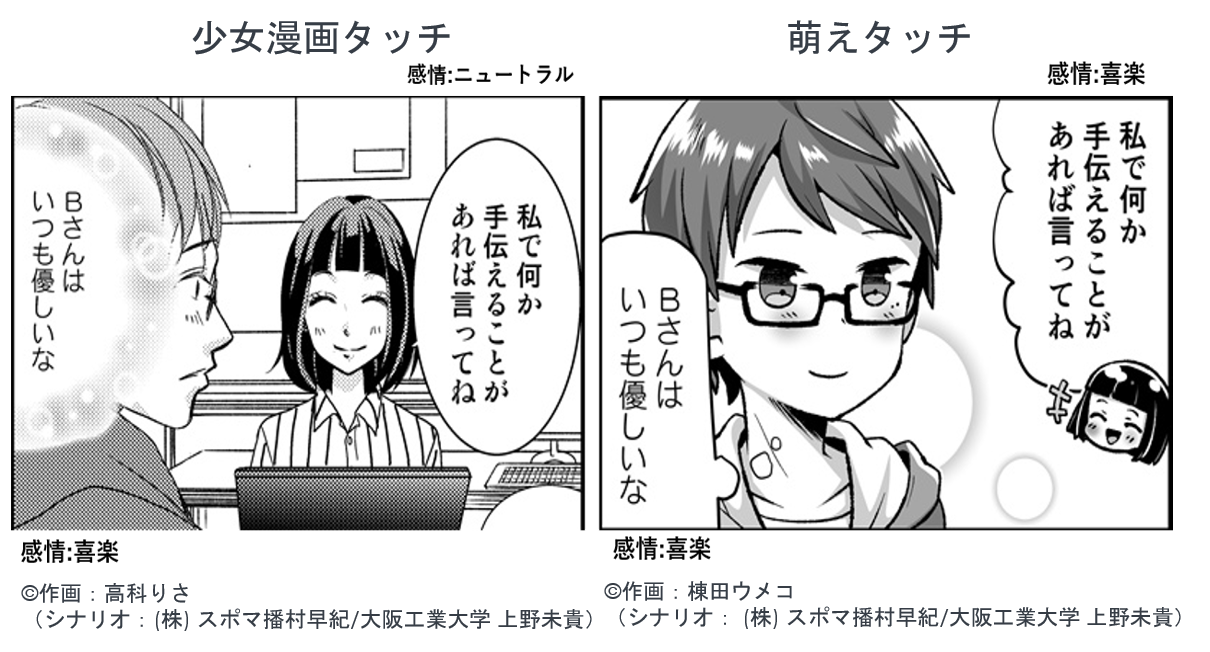
\includegraphics[width=\linewidth]{4koma.png}
  \caption{タッチごとのアノテート例}
  \label{fig:4koma}
\end{figure}

\section{要素技術}
\subsection{BERT}
BERT (Bidirectional Encoder Representations from Transformers)\cite{BERT} は 2018 年に Google が発表した言語モデルの一種である.

その名前の通り,Transformer により構成される双方向のエンコーダであり, 文書分類や質疑応答といった様々な自然言語処理の幅広いタスクにおいて公開時点での最高性能を達成している.
従来のニューラルネットワークを用いた自然言語処理モデルは, 特定のタスクに対して 1 つのモデルを用いてきたが, BERT は転移学習により, 1 つのモデルで, 様々なタスクに対応できる. また, BERTを転移学習したモデルは, 少ないデータを追加学習するのみで動作するため, 1 からモデルを構築しなくて済む. 本稿では日本語 Wikipedia より全 1800 万文を用いて事前学習させたモデル\footnote{\url{http://nlp.ist.i.kyoto-u.ac.jp/index.php}} と
大規模日本語 SNS コーパスによってモデル事前学習させたモデル \cite{hottoSNS-bert} を用いた.
を用いた.
\newpage

\subsection{illustration2vec}
illustration2vec \cite{i2v} は Saito, Matsui らが提案した画像のベクトル化手法であり, Danbooru と Safebooru から 100 万枚のイラストを用いて学習した事前学習済みモデルが公開されている. illustration2vec が扱った問題として, イラストに対する画像認識の難しさがあり, 既存の画像認識モデルのほとんどが ImageNet などの実画像を評価対象にしており, アニメや漫画といったイラストに対して評価をしていなかった. illustration2vec はそれらと比較してイラストのより合理的なベクトル化が期待できる手法である. 本稿では事前学習済みモデルを使って 4096 次元のコマ画像のベクトルを獲得する.

\section{Data Augmentation}
4 コマ漫画ストーリーデータセットの欠点として, データ数が少ないことがあげられる. そこで, 本実験では日本語 WordNet \cite{word_net_jp} のシソーラスを用いてテキストデータを拡張する.
分かち書きされたオリジナルのセリフに対して, 日本語 WordNet で類似語を持つ単語について類似語に置き換え, 文を生成することでテキストデータを拡張した. ただし, 文の中に類義語を持つ単語が
複数あった場合, 類似語に置き換える単語は同時に 1 つまでとし, 英数字・記号のみで表されている類似語は除外した. 例えば, 5 つの単語からなる文章があり,
各単語が 5 つの類似語を持っている場合, その文からは新しく 25 文が生成されることとなる.

\section{実験}
本稿では, 各タッチについての感情推定を行った.
使用するデータセットには 7 種類の感情ラベル(ニュートラル, 驚愕, 喜楽, 恐怖, 悲哀, 憤怒, 嫌悪)と, アノテーション不備によるラベル不明 (以下, ``UNK" とする) の全 8 種類
が含まれているが, データ数と解析の難しさの問題から, 今回は喜楽のみを正例, その他を負例とする 2 クラスに分類した.

訓練用データは各タッチの前半 1 話から 5 話までの拡張されたセリフを用い,
評価用データは後半 6 話から 10 話におけるオリジナルのセリフのみを用いた.
表\ref{table:data_size}に各実験で用いたデータ数を示す.

多くのタッチにおいて, 正例は負例に対してデータ数が非常に少ない不均衡データであることから, 損失関数に使うクラス重みとして各タッチについて, 訓練用データの各ラベルのデータ数の逆数を正規化したものを用いた. また, 訓練用データの内 20 \% をサンプリングして検証用データとし, 検証用データにおける正例の F1 値が最大となる epoch のものを評価用モデルとして採用してモデルの性能を測った.

\begin{table}[t]
\centering
\caption{データ数}
\label{table:data_size}
\scalebox{0.7}{
\begin{tabular}{|c|l||c|c|c|c|c|}
\hline
\multicolumn{1}{|l|}{\textbf{}}                      & \textbf{ラベル} & \multicolumn{1}{l|}{\textbf{ギャグ}} & \multicolumn{1}{l|}{\textbf{少女}} & \multicolumn{1}{l|}{\textbf{少年}} & \multicolumn{1}{l|}{\textbf{青年}} & \multicolumn{1}{l|}{\textbf{萌え}} \\ \hline
\multirow{4}{*}{\textbf{train\&valid}}                 & 喜楽        & 15                                & 39                               & 15                               & 18                               & 25                                \\ \cline{2-7}
                                                     & その他       & 40                                & 26                               & 45                               & 44                               & 35                                \\ \cline{2-7}
                                                     & 喜楽(拡張後)   & 1115                              & 2575                             & 940                              & 998                              & 1766                              \\ \cline{2-7}
                                                     & その他(拡張後)  & 2851                              & 1391                             & 3076                             & 3145                             & 2323                              \\ \hline
\multicolumn{1}{|l|}{\multirow{2}{*}{\textbf{test}}} & 喜楽        & 10                                & 38                               & 12                               & 14                               & 22                                \\ \cline{2-7}
\multicolumn{1}{|l|}{}                               & その他       & 56                                & 29                               & 52                               & 51                               & 42                                \\ \hline
\end{tabular}
}
\end{table}

\subsection{\small{実験 1 : セリフ 1 文の感情推定}}
実験 1 では 1 つのセリフを入力し, 対応する感情ラベルを出力するような感情推定をした. JUMAN++ \footnote{http://nlp.ist.i.kyoto-u.ac.jp/index.php?JUMAN++} によって分かち書きされたセリフをさらにサブワード化したものを BERT への入力とし, 識別器としては 3 層 MLP を用いた. 表\ref{table:mlp_para}に MLP で用いたパラメータ, そして表\ref{table:ex_para}に学習で用いたパラメータを示す. 学習率は Optuna\cite{optuna_2019} によって最適なパラメータを探索した.

BERT の事前学習済みモデルの全ての重みを固定した場合 (BERT fixed) と最終層のパラメータだけをチューニングした場合 (BERT last layer) の 2 つの手法について感情推定をして, 各タッチ・手法の結果について比較し, fine tuning の有用性を確かめた.

\begin{table}[htb]
\caption{実験 1 MLP パラメータ}
\label{table:mlp_para}
\centering
\begin{tabular}{|c||c|c|}
\hline
parameters & MLP \\ \hline
(in,hidden,out) & (768,30,2) \\ \hline
activation function & tanh \\ \hline
dropout rate & 0.5 \\ \hline
\end{tabular}
\end{table}

\begin{table}[htb]
\caption{学習パラメータ}
\label{table:ex_para}
\centering
\begin{tabular}{|c||c|c|}
\hline
parameters & \multicolumn{2}{|c|}{実験 $1・2・3$} \\ \hline
epoch & \multicolumn{2}{|c|}{200}  \\ \hline
batch size & \multicolumn{2}{|c|}{16} \\ \hline
loss function & \multicolumn{2}{|c|}{Cross Entropy Loss} \\ \hline
optimizer & \multicolumn{2}{|c|}{Adam} \\ \hline
\end{tabular}
\end{table}

\newpage

\subsection{\small{実験 2 : 過去のセリフを考慮した感情推定}}
実験 2 では, 連続したセリフ $n$ 文を入力し, 末尾のセリフに対応する感情ラベルを出力する感情推定をした.
図\ref{fig:net} に $n = 3$ とした時のネットワークの概略図を示す. $\{s_i\}$ はそれぞれ連続する $n$ 文のセリフを BERT の 単語 ID 列に変換したものである. 単語 ID 列はセリフ内の最大単語長に合わせて, 後方パディングをしている. また, 4 コマ漫画ストーリーデータセットは 1 話につき 2 つの 4 コマを含んでいるが, 各 4 コマは時系列的に繋がっていないことを踏まえて, ${s_i}$ のセリフの組み合わせとしては同一の 4 コマに属し, かつ連続しているものを扱う. 各 4 コマの序盤に現れるセリフには参照できる過去のセリフが無いため, 便宜上のセリフ ``$[$pad$]$" を置くことで対処した. 末尾のセリフ以外はオリジナルのセリフのみから抽出し, すべての組み合わせを入力列とすることで, 実験 1 のデータ数と合わせた.

単語 ID 列長を $w$ とすると入力次元は $(batch \times n \times w)$ となる. このままでは BERT の入力次元に対応していないので, まず $(n \times batch \times w)$ へと軸を入れ替え, これを 1 次元目について各ベクトルに分解し, これら $n$ 個の 次元数 $(batch \times w)$ のベクトルをそれぞれ BERT への入力とし, BERT の出力から [CLS] トークンに相当するベクトルのみをそれぞれ抜き取り, 先と逆の手順を踏むことで次元数 $(batch \times n \times 768)$ のテンソルを得る. これを識別器として用いる Bi-LSTM をベースとした Self-Attention への入力とすることで末尾のセリフの感情を推定するように学習を行う. 本稿では $n$ を 2 から 6 に変えて実験した.

BERT は最終層のみをチューニングする. 学習で用いたパラメータは表\ref{table:ex_para}, 識別器のパラメータは表\ref{tab:self_net} に示す.

\begin{figure}[!htb]
  \begin{center}
    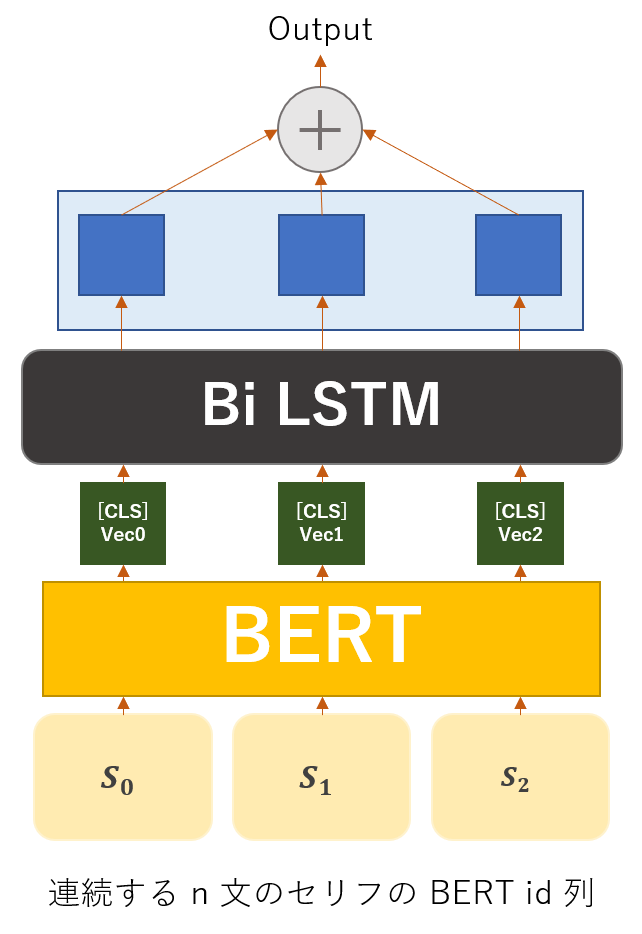
\includegraphics[scale=0.5]{seq_net.png}
    \caption{提案ネットワーク ($n = 3$)} %タイトルをつける
    \label{fig:net} %ラベルをつけ図の参照を可能にする
  \end{center}
\end{figure}

\begin{table}[bht]
\begin{center}
\caption{実験 2 識別器パラメータ}
\begin{tabular}{|c|c|}
\hline
parameters & value \\ \hline
lstm\_in & 768   \\ \hline
lstm\_hidden    & 128    \\ \hline
self\_atten\_in & $128 \times 2$   \\ \hline
atten\_num\_layers & 3     \\ \hline
\end{tabular}
\label{tab:self_net}
\end{center}
\end{table}

\subsection{\small{実験 3 : マルチモーダルな感情推定の検討}}
実験 1 と同様にして, BERT の事前学習済みモデルの全ての重みを固定した場合 (BERT fixed) と最終層のパラメータだけをチューニングした場合 (BERT last layer) の 2 つの手法について BERT から得た 768 次元のベクトルと, 入力したセリフが含まれているコマ全体の画像を illustration2vec に入力して得た 4096 次元のベクトルを concat した 4864 次元のベクトルを入力ベクトルとして, 3 層 MLP に入力することでマルチモーダルな感情推定をした. データセット整備の都合上, 本稿では少年漫画タッチ, 青年漫画タッチ, 萌えタッチについてのみ実験をした.

\section{実験結果}
実験 1, 2, 3 において, すべての出力が負例と推定された場合の評価指標の値をベースラインとして設定した. 以下, 表における P-Recall, P-F1 値は正例の再現率, F1 値を表し, Acc は全体の精度を表す. また, Recall が 0 の時の F1 値は 0 とした. 5 タッチ総合の結果は各タッチにおける混合行列の和から算出してある.

\subsection{実験 1 : 結果}
表\ref{table:result_1}に実験 1 の結果を示す.
表\ref{table:result_1}より, Accuracy に関しては差異はないが共にベースラインを超え, P-Recall, P-F1 値共に BERT fixed より BERT last layer の方が上だったことから, fine tuning の有用性を確かめることができた.

\subsection{実験 2 : 結果}
表\ref{table:result_2}に実験 2 の結果を示す.
表\ref{table:result_2}より, 実験 1 と比べ, 全体的に評価指標は下回ったことから, 過去のセリフを考慮することの優位性を示すことはできなかったが, $n$ が大きくなるに従って P-F1 値は増加傾向にあることから過去のセリフをより多く考慮することの有用性はあると推測できる. しかし, $n$ が 4 以上の場合, 各評価指標の値に差異は見られない. これは 4 コマ漫画という性質上, 4 コマ内に含まれるセリフの数は十分に少ないことから, $n$ を増やしても ``$[$pad$]$" が入力列に増えるだけの場合が多いことに起因すると考えられる.

\subsection{実験 3 : 結果}
表\ref{table:result_3}に実験 3 の結果を示す. 比較として, 実験 1 における 3 タッチの結果も合わせて載せている.
表\ref{table:result_3}より, 実験 1 と比べ, P-Recall 以外の評価指標は下回ったものの, 少年漫画タッチにおいては実験 1 と実験 2 と比較すると最も高い P-Recall と P-F1 値が得られており, マルチモーダルな感情推定の意味があると考えられる.


\section{考察}
まず, 各実験の結果についての考察を述べる. 過去のセリフを考慮することで 実験 2 において, 全体的に評価指標が下回ったのは, ネットワークの柔軟性が上がり, より過学習が進んだことで汎化性能が下がったことが原因だと考えられる. Optuna で探索する学習率の範囲は共通しており, 学習曲線を見ても実験 2 の方がより早く収束している場合が多かったことから, 柔軟性に合わせて探索範囲を変えたり, 学習率スケジューラーを設定したり, 適宜 Dropout 層を追加するなどをして過学習を抑制する必要があると考えられる. 実験 3 においても同様のことが言えるが, コマの画像ベクトルがセリフの分散表現に対して次元数がかなり多いことを踏まえると, 全結合層などを追加し, 次元数を合わせる必要もあると考えられる. ただし, illustration2vec のモデルがこの実験に適しているかの妥当性は確認していないため, これは今後の課題である.

次に, データ及びモデルの問題点について考察する. 本稿では Data Augmentation の手法における, 文法的齟齬の問題については取り組んでおらず, この問題がどれだけ寄与しているかについての調査は今後の課題である. 具体的な解決策としては, 拡張されたセリフの分散表現とそれぞれに対応するオリジナルのセリフの分散表現とのコサイン類似度から閾値未満のデータを除外したり, 拡張する品詞を限定するといったことが考えられる. また, 本稿で用いた BERT の事前学習済みモデルでは, `!' や `?' 等の記号は未知語として扱われており, 漫画においてはこれらの記号がニュートラル以外の感情を表す表現として使われるという経験則があることや, 実際にデータの中にこれらの記号のみで構成されてニュートラル以外の感情ラベルが付与されているセリフがあることなどこれらの記号を適切に処理する方法を考える必要がある. 具体的にはこれらの記号を特殊なトークンに置き換えて学習させたり, またはこれらの記号が辞書に含まれている他の事前学習済みモデルを用いるなどがあり, その精度も合わせて比較したい. そして, そもそものデータ数が極めて少ない問題の解決も重要な課題である.

\section{まとめと今後の課題}
本稿では BERT で得たセリフの分散表現からセリフの感情の推定をした. 実験結果から過去のセリフを考慮することの優位性を示すには多くの課題があることが分かった. また, コマの画像のベクトルも考慮したマルチモーダルな感情推定もしたが, 1 つのセリフを入力とする実験では優位性は見られなかった. 時系列を考慮したセリフのマルチモーダルな感情推定は実験 2 において入力したそれぞれのセリフが含まれているコマ全体の画像のベクトルを BERT からの出力にそれぞれ concat すれば可能であるから, 今後の課題とする.

今後の課題として, 4 コマ漫画ストーリーデータセットのみでの訓練・テストでは精度の向上が困難であることから, 何かしらの日本語の極性評価データセットを用いて BERT の事前学習モデルを fine tuning し, 4 コマ漫画の感情推定問題に転移させることが考えられる. 場合によっては感情ラベルの貼り直し, または人手によるラベル付けが必要になる. また Manga 109 のセリフのデータを用いることで半教師あり学習も可能であり, マルチモーダルな感情推定手法についても更なる工夫が必要である.


\begin{table*}[!b]
\begin{center}
\caption{実験 1 結果(評価用データ)}
\label{table:result_1}
\scalebox{0.61}{
\begin{tabular}{cccccccccccccccc|ccc}
  \hline
  \multirow{2}{*}{} & \multicolumn{3}{c}{ギャグ} & \multicolumn{3}{c}{少女漫画} & \multicolumn{3}{c}{少年漫画} & \multicolumn{3}{c}{青年漫画} & \multicolumn{3}{c|}{萌え} & \multicolumn{3}{c}{5タッチ総合} \\
   & Acc & P-Recall & P-F1 & Acc & P-Recall & P-F1 & Acc & P-Recall & P-F1 & Acc & P-Recall & P-F1 & Acc & P-Recall & P-F1 & Acc & P-Recall & P-F1 \\ \hline
  BERT fixed & 0.757 & 0.200 & 0.200 & 0.552 & 0.684 & 0.634 & 0.796 & 0.000 & 0.000 & 0.784 & 0.357 & 0.416 & 0.718 & 0.454 & {\bf 0.526} & 0.720 & 0.447 & 0.485 \\
  BERT last layer & 0.818 & 0.200 & {\bf 0.250} & 0.641 & 0.710 & {\bf 0.692} & 0.781 & 0.000 & 0.000 & 0.800 & 0.500 & {\bf 0.518} & 0.578 & 0.500 & 0.448 & 0.723 & 0.489 & {\bf 0.510} \\ \hline
  ベースライン & \multicolumn{1}{l}{0.848} & 0.000 & 0.000 & 0.432 & 0.000 & 0.000 & 0.812 & 0.000 & 0.000 & 0.784 & 0.000 & 0.000 & 0.656 & 0.000 & 0.000 & 0.705 & 0.000 & 0.000
\end{tabular}
}
\end{center}
\end{table*}

% \begin{figure*}[t]
%   \centering
%   \includegraphics[width=\linewidth]{ex2_graph_shounen.png}
%   \caption{実験 2 学習推移 (少年漫画タッチ 時系列長 $\rm N = 6$)}
%   \label{fig:ex2_graph}
% \end{figure*}

\begin{table*}[!b]
\begin{center}
\caption{実験 2 結果(評価用データ)}
\scalebox{0.61}{
\begin{tabular}{cccccccccccccccc|ccc}
  \hline
  \multirow{2}{*}{n} & \multicolumn{3}{c}{ギャグ} & \multicolumn{3}{c}{少女漫画} & \multicolumn{3}{c}{少年漫画} & \multicolumn{3}{c}{青年漫画} & \multicolumn{3}{c|}{萌え} & \multicolumn{3}{c}{5タッチ総合} \\
   & Acc & P-Recall & P-F1 & Acc & P-Recall & P-F1 & Acc & P-Recall & P-F1 & Acc & P-Recall & P-F1 & Acc & P-Recall & P-F1 & Acc & P-Recall & P-F1 \\ \hline
  2 & 0.803 & 0.200 & 0.235 & 0.492 & 0.526 & 0.540 & 0.765 & 0.083 & 0.117 & 0.738 & 0.285 & 0.320 & 0.578 & 0.363 & 0.372 & 0.674 & 0.364 & 0.397 \\
  3 & 0.772 & 0.000 & 0.000 & 0.626 & 0.526 & 0.615 & 0.765 & 0.000 & 0.000 & 0.800 & 0.285 & 0.380 & 0.625 & 0.409 & 0.428 & 0.717 & 0.343 & 0.417 \\
  4 & 0.772 & 0.000 & 0.000 & 0.582 & 0.578 & 0.611 & 0.781 & 0.083 & 0.125 & 0.769 & 0.571 & {\bf 0.516} & 0.546 & 0.681 & {\bf 0.508} & 0.687 & 0.479 & 0.474 \\
  5 & 0.742 & 0.500 & {\bf 0.370} & 0.641 & 0.552 & 0.636 & 0.781 & 0.000 & 0.000 & 0.769 & 0.428 & 0.444 & 0.625 & 0.500 & 0.478 & 0.711 & 0.447 & 0.477 \\
  6 & 0.787 & 0.100 & 0.125 & 0.611 & 0.657 & {\bf 0.657} & 0.812 & 0.083 & {\bf 0.142} & 0.753 & 0.285 & 0.333 & 0.562 & 0.590 & 0.481 & 0.705 & 0.458 & {\bf 0.478} \\ \hline
  ベースライン & \multicolumn{1}{l}{0.848} & 0.000 & 0.000 & 0.432 & 0.000 & 0.000 & 0.812 & 0.000 & 0.000 & 0.784 & 0.000 & 0.000 & 0.656 & 0.000 & 0.000 & 0.705 & 0.000 & 0.000
\end{tabular}
\label{table:result_2}
}
\end{center}
\end{table*}


\begin{table*}[!b]
\begin{center}
\caption{実験 3 結果(評価用データ)}
\label{table:result_3}
\scalebox{0.59}{
\begin{tabular}{lcccccccccccccccc|ccc}
  \hline
   & \multirow{2}{*}{} & \multicolumn{3}{c}{ギャグ} & \multicolumn{3}{c}{少女漫画} & \multicolumn{3}{c}{少年漫画} & \multicolumn{3}{c}{青年漫画} & \multicolumn{3}{c|}{萌え} & \multicolumn{3}{c}{3 タッチ平均} \\
   &  & Acc & P-Recall & P-F1 & Acc & P-Recall & P-F1 & Acc & P-Recall & P-F1 & Acc & P-Recall & P-F1 & Acc & P-Recall & P-F1 & Acc & P-Recall & P-F1 \\ \hline
  \multirow{2}{*}{実験 1} & BERT fixed & - & - & - & - & - & - & 0.796 & 0.000 & 0.000 & 0.784 & 0.357 & 0.416 & 0.718 & 0.454 & {\bf 0.526} & 0.766 & 0.312 & {\bf 0.400} \\
   & BERT last layer & - & - & - & - & - & - & 0.781 & 0.000 & 0.000 & 0.800 & 0.500 & {\bf 0.518} & 0.578 & 0.500 & 0.448 & 0.720 & 0.375 & {\bf 0.400} \\ \hline
  \multirow{2}{*}{実験 3} & BERT fixed & - & - & - & - & - & - & 0.328 & 0.750 & 0.295 & 0.446 & 0.571 & 0.307 & 0.546 & 0.409 & 0.382 & 0.440 & 0.520 & 0.316 \\
   & \multicolumn{1}{l}{BERT last layer} & - & - & - & - & - & - & 0.562 & 0.500 & {\bf 0.300} & 0.784 & 0.500 & 0.500 & 0.562 & 0.363 & 0.363 & 0.637 & 0.437 & 0.375 \\ \hline
   & ベースライン & - & - & - & - & - & - & 0.812 & 0.000 & 0.000 & 0.784 & 0.000 & 0.000 & 0.656 & 0.000 & 0.000 & 0.751 & 0.000 & 0.000
\end{tabular}
}
\end{center}
\end{table*}

\bibliographystyle{unsrt}
\bibliography{sankou}
\end{document}
